\chapter{Probabilités conditionnelles et indépendance}\label{ch:g12:condprob}

La \omterm{def:g10:proba:distribution}{probabilité} quantifie l'incertitude~; la \omterm{def:g12:condprob:cond}{probabilité conditionnelle}
quantifie comment l'information la modifie. Apprendre qu'un \omterm{def:g11:prob:model}{événement} $B$
s'est produit remodèle les \omterm{def:g10:proba:distribution}{probabilités} de tous les autres \omterm{def:g11:prob:model}{événements} ---
un mécanisme formalisé par Bayes et mal utilisé chaque jour dans les
tribunaux et les journaux. Ce chapitre met en place les règles du
conditionnement et le sens exact de l'\omterm{def:g12:condprob:indep}{indépendance}.

\section{Espaces de probabilité (rappel)}

Une expérience à un nombre fini d'issues se modélise par un \emph{\omterm{def:g11:prob:model}{univers}}
$\Omega$ (l'ensemble des issues) et une \omterm{def:g10:proba:distribution}{probabilité} $\P$ associant à chaque
\omterm{def:g11:prob:model}{événement} $A \subseteq \Omega$ un nombre $\P(A) \in \intcc{0}{1}$, additive
sur les unions disjointes et avec $\P(\Omega) = 1$. Rappeler les règles de
base~:
\[
\P(\bar A) = 1 - \P(A),
\qquad
\P(A \cup B) = \P(A) + \P(B) - \P(A \cap B).
\]
Lorsque toutes les issues sont équiprobables,
$\P(A) = \frac{\abs A}{\abs\Omega}$ --- et le calcul des \omterm{def:g10:proba:distribution}{probabilités} se
réduit aux techniques de dénombrement du \cref{ch:g12:comb}.

\section{Probabilité conditionnelle}

\begin{definition}[Probabilité conditionnelle]\label{def:g12:condprob:cond}
Soit $B$ un \omterm{def:g11:prob:model}{événement} avec $\P(B) > 0$. La \emph{probabilité de $A$ sachant
$B$}\index{probabilité conditionnelle} est
\[
\pcond{B}{A} = \frac{\P(A \cap B)}{\P(B)} .
\]
\end{definition}

L'application $A \mapsto \pcond BA$ est elle-même une \omterm{def:g10:proba:distribution}{probabilité} (toutes
les règles s'appliquent)~; elle représente le nouvel état de connaissance de
quelqu'un qui a appris que $B$ s'est produit.

\begin{proposition}[Règle de multiplication]\label{prop:g12:condprob:product}
Pour des \omterm{def:g11:prob:model}{événements} de \omterm{def:g10:proba:distribution}{probabilités} non nulles~:
\[
\P(A \cap B) = \P(B)\,\pcond{B}{A} = \P(A)\,\pcond{A}{B},
\]
et plus généralement
$\P(A_1 \cap A_2 \cap A_3) = \P(A_1)\,\pcond{A_1}{A_2}\,
\pcond{A_1 \cap A_2}{A_3}$, etc.
\end{proposition}

\begin{proof}
Réarranger la définition~; la formule en chaîne suit par itération.
\end{proof}

\begin{theorem}[Formule des probabilités totales]\label{thm:g12:condprob:total}
\index{formule des probabilités totales}
Soient $B_1, \dots, B_n$ une partition de $\Omega$ en \omterm{def:g11:prob:model}{événements} de
\omterm{def:g10:proba:distribution}{probabilité} non nulle. Pour tout \omterm{def:g11:prob:model}{événement} $A$~:
\[
\P(A) = \sum_{i=1}^{n} \P(B_i)\,\pcond{B_i}{A}.
\]
\end{theorem}

\begin{proof}
Les ensembles $A \cap B_i$ sont deux à deux disjoints d'union $A$, donc
$\P(A) = \sum_i \P(A \cap B_i) = \sum_i \P(B_i)\pcond{B_i}{A}$ par la règle
de multiplication.
\end{proof}

\begin{method}[Arbres de probabilité]\label{met:g12:condprob:tree}
Un \omterm{met:g10:proba:tree}{arbre} organise les \omterm{def:g12:condprob:cond}{probabilités conditionnelles}~: chaque branche porte
la \omterm{def:g10:proba:distribution}{probabilité} de l'\omterm{def:g11:prob:model}{événement} suivant \emph{sachant} le chemin déjà parcouru.
\begin{itemize}
  \item La \omterm{def:g10:proba:distribution}{probabilité} d'une feuille (un chemin complet) est le
        \emph{produit} des \omterm{def:g10:proba:distribution}{probabilités} le long de ses branches (règle de
        multiplication).
  \item La \omterm{def:g10:proba:distribution}{probabilité} d'un \omterm{def:g11:prob:model}{événement} est la \emph{somme} des \omterm{def:g10:proba:distribution}{probabilités}
        des feuilles qui le réalisent (\omterm{def:g10:proba:distribution}{probabilités} totales).
  \item Les \omterm{def:g10:proba:distribution}{probabilités} des branches issues d'un nœud s'additionnent à $1$.
\end{itemize}
\end{method}

\begin{omfigure}
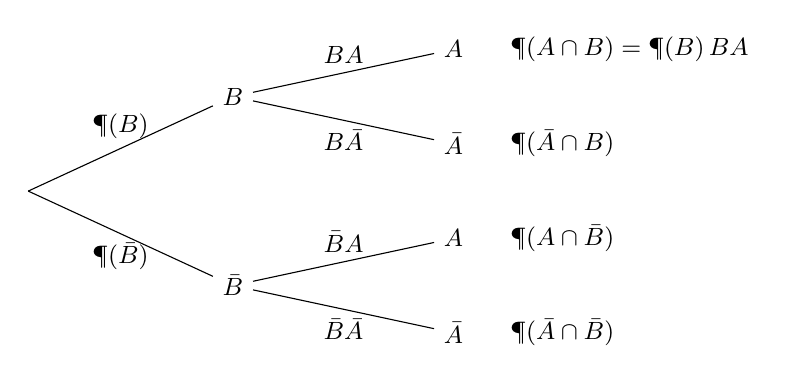
\begin{tikzpicture}[font=\small]
  \coordinate (root) at (0,0);
  \node (B)  at (2.6,1.2)  {$B$};
  \node (Bc) at (2.6,-1.2) {$\bar B$};
  \node (BA)  at (5.4,1.8)  {$A$};
  \node (BAc) at (5.4,0.6)  {$\bar A$};
  \node (BcA)  at (5.4,-0.6) {$A$};
  \node (BcAc) at (5.4,-1.8) {$\bar A$};
  \draw (root) -- (B)  node[midway, above] {$\P(B)$};
  \draw (root) -- (Bc) node[midway, below] {$\P(\bar B)$};
  \draw (B) -- (BA)   node[midway, above] {$\pcond{B}{A}$};
  \draw (B) -- (BAc)  node[midway, below] {$\pcond{B}{\bar A}$};
  \draw (Bc) -- (BcA)  node[midway, above] {$\pcond{\bar B}{A}$};
  \draw (Bc) -- (BcAc) node[midway, below] {$\pcond{\bar B}{\bar A}$};
  \node[anchor=west] at (6.0,1.8)  {$\P(A \cap B) = \P(B)\,\pcond{B}{A}$};
  \node[anchor=west] at (6.0,0.6)  {$\P(\bar A \cap B)$};
  \node[anchor=west] at (6.0,-0.6) {$\P(A \cap \bar B)$};
  \node[anchor=west] at (6.0,-1.8) {$\P(\bar A \cap \bar B)$};
\end{tikzpicture}

{\small Un \omterm{met:g10:proba:tree}{arbre} à deux niveaux~: multiplier le long d'un chemin, additionner
sur les feuilles. Par exemple $\P(A)$ est la somme des \omterm{def:g10:proba:distribution}{probabilités} des
première et troisième feuilles.}
\end{omfigure}

\begin{theorem}[Formule de Bayes]\label{thm:g12:condprob:bayes}
\index{formule de Bayes}
Soient $B_1, \dots, B_n$ une partition de $\Omega$ comme ci-dessus et $A$
un \omterm{def:g11:prob:model}{événement} avec $\P(A) > 0$. Alors
\[
\pcond{A}{B_j} =
\frac{\P(B_j)\,\pcond{B_j}{A}}{\sum_{i=1}^{n} \P(B_i)\,\pcond{B_i}{A}} .
\]
\end{theorem}

\begin{proof}
$\pcond{A}{B_j} = \frac{\P(A \cap B_j)}{\P(A)}$~; \omterm{def:g10:algebra:expand}{développer} le numérateur
par la règle de multiplication et le dénominateur par les \omterm{def:g10:proba:distribution}{probabilités}
totales.
\end{proof}

\begin{example}[Test de dépistage]\label{ex:g12:condprob:test}
Une maladie touche $1\%$ d'une population. Un test la détecte avec
\omterm{def:g10:proba:distribution}{probabilité} $0.99$ (sensibilité) et donne un faux positif avec \omterm{def:g10:proba:distribution}{probabilité}
$0.05$. Sachant un test positif, la \omterm{def:g10:proba:distribution}{probabilité} d'avoir effectivement la
maladie est
\[
\frac{0.01 \times 0.99}{0.01\times0.99 + 0.99\times0.05}
= \frac{0.0099}{0.0099 + 0.0495} = \frac{1}{6} \approx 0.17 .
\]
Malgré le test précis, cinq positifs sur six sont des faux --- parce que la
maladie est rare. Confondre $\pcond{A}{B}$ avec $\pcond{B}{A}$ est le
\emph{sophisme du procureur}.
\end{example}

\begin{omfigure}
\begin{tikzpicture}[font=\small]
  \coordinate (root) at (0,0);
  \node (D)  at (2.6,1.2)  {$D$};
  \node (Dc) at (2.6,-1.2) {$\bar D$};
  \node (DT)  at (5.2,1.8)  {$T$};
  \node (DTc) at (5.2,0.6)  {$\bar T$};
  \node (DcT)  at (5.2,-0.6) {$T$};
  \node (DcTc) at (5.2,-1.8) {$\bar T$};
  \draw (root) -- (D)  node[midway, above] {$0.01$};
  \draw (root) -- (Dc) node[midway, below] {$0.99$};
  \draw (D) -- (DT)   node[midway, above] {$0.99$};
  \draw (D) -- (DTc)  node[midway, below] {$0.01$};
  \draw (Dc) -- (DcT)  node[midway, above] {$0.05$};
  \draw (Dc) -- (DcTc) node[midway, below] {$0.95$};
  \node[omThm, anchor=west] at (5.8,1.8)  {$0.0099$ \ (vrais positifs)};
  \node[anchor=west] at (5.8,0.6)  {$0.0001$};
  \node[omThm, anchor=west] at (5.8,-0.6) {$0.0495$ \ (faux positifs)};
  \node[anchor=west] at (5.8,-1.8) {$0.9405$};
\end{tikzpicture}

{\small Le test de dépistage en \omterm{met:g10:proba:tree}{arbre} ($D$~: malade, $T$~: test positif).
Les deux feuilles positives (en rouge) ont un poids total $0.0594$, dont
les faux positifs contribuent pour les cinq sixièmes.}
\end{omfigure}

\section{Indépendance}

\begin{definition}[Événements indépendants]\label{def:g12:condprob:indep}
Deux \omterm{def:g11:prob:model}{événements} $A$ et $B$ sont \emph{indépendants}\index{indépendance} si
\[
\P(A \cap B) = \P(A)\,\P(B) .
\]
Lorsque $\P(B) > 0$, cela équivaut à $\pcond{B}{A} = \P(A)$~: savoir $B$ ne
change pas la \omterm{def:g10:proba:distribution}{probabilité} de $A$.
\end{definition}

\begin{proposition}\label{prop:g12:condprob:indepcompl}
Si $A$ et $B$ sont \omterm{def:g12:condprob:indep}{indépendants}, il en va de même de $A$ et $\bar B$ (et de
$\bar A$ et $\bar B$).
\end{proposition}

\begin{proof}
$\P(A \cap \bar B) = \P(A) - \P(A \cap B) = \P(A) - \P(A)\P(B)
= \P(A)\bigl(1 - \P(B)\bigr) = \P(A)\,\P(\bar B)$.
\end{proof}

\begin{remark}
Ne pas confondre \emph{\omterm{def:g12:condprob:indep}{indépendants}} ($\P(A\cap B) = \P(A)\P(B)$) et
\emph{\omterm{def:g10:proba:operations}{incompatibles}} ($A \cap B = \varnothing$). Deux \omterm{def:g11:prob:model}{événements}
\omterm{def:g10:proba:operations}{incompatibles} de \omterm{def:g10:proba:distribution}{probabilité} non nulle ne sont jamais \omterm{def:g12:condprob:indep}{indépendants}~: savoir
que l'un s'est produit garantit que l'autre ne s'est pas produit.
\end{remark}

\begin{definition}[Répétitions indépendantes]\label{def:g12:condprob:repet}
Lorsqu'une expérience est répétée $n$ fois de sorte que l'issue de chaque
épreuve n'influence pas les autres, la \omterm{def:g10:proba:distribution}{probabilité} d'une \omterm{def:g12:seq:sequence}{suite} spécifiée
d'issues est le produit des \omterm{def:g10:proba:distribution}{probabilités} individuelles. C'est le modèle
sous-jacent à la \omterm{def:g11:prob:rv}{loi} binomiale (\cref{ch:g12:randvar}).
\end{definition}

\section{Exercices}

\begin{exercise}[$\star$]\label{exo:g12:condprob:1}
On tire une carte d'un jeu standard de 52 cartes. Calculer la \omterm{def:g10:proba:distribution}{probabilité}
que ce soit un roi, sachant que c'est une figure (valet, dame ou roi). Les
\omterm{def:g11:prob:model}{événements} «~roi~» et «~cœur~» sont-ils \omterm{def:g12:condprob:indep}{indépendants}~?
\end{exercise}

\begin{exercise}[$\star$]\label{exo:g12:condprob:2}
Une urne contient 5 boules rouges et 3 bleues. On tire deux boules à la
\omterm{def:g12:seq:sequence}{suite} \emph{sans} remise.
\begin{enumerate}
  \item Dessiner l'\omterm{met:g10:proba:tree}{arbre} de \omterm{def:g10:proba:distribution}{probabilité}.
  \item Calculer la \omterm{def:g10:proba:distribution}{probabilité} que les deux soient rouges, et la
        \omterm{def:g10:proba:distribution}{probabilité} que la seconde soit rouge.
\end{enumerate}
\end{exercise}

\begin{exercise}[$\star$]\label{exo:g12:condprob:3}
On lance deux dés équilibrés. Soient $A$ = «~la somme vaut $7$~», $B$ =
«~le premier dé montre $3$~», $C$ = «~la somme vaut $6$~». Déterminer si $A$
et $B$ sont \omterm{def:g12:condprob:indep}{indépendants}, puis si $B$ et $C$ le sont.
\end{exercise}

\begin{exercise}[$\star\star$]\label{exo:g12:condprob:4}
Une usine a trois machines produisant respectivement $50\%$, $30\%$ et
$20\%$ de la production totale, avec des taux de défaut $1\%$, $2\%$ et
$4\%$.
\begin{enumerate}
  \item Quelle proportion de la production est défectueuse~?
  \item Un article tiré au hasard est défectueux. Quelle est la \omterm{def:g10:proba:distribution}{probabilité}
        qu'il vienne de la troisième machine~?
\end{enumerate}
\end{exercise}

\begin{exercise}[$\star\star$]\label{exo:g12:condprob:5}
Dans l'\cref{ex:g12:condprob:test}, pour quelle prévalence $p$ de la maladie
(au lieu de $1\%$) un test positif signifierait-il au moins $90\%$ de chance
d'être malade~? Résoudre l'inégalité et commenter.
\end{exercise}

\begin{exercise}[$\star\star$]\label{exo:g12:condprob:6}
Une pièce biaisée tombe sur pile avec \omterm{def:g10:proba:distribution}{probabilité} $p \in \intoo{0}{1}$. On
la lance trois fois, les lancers étant \omterm{def:g12:condprob:indep}{indépendants}.
\begin{enumerate}
  \item Calculer la \omterm{def:g10:proba:distribution}{probabilité} de l'\omterm{def:g11:prob:model}{événement} $E$ = «~exactement deux
        piles~».
  \item Pour quels $p$ la quantité $\P(E)$ est-elle maximale~?
\end{enumerate}
\end{exercise}

\begin{exercise}[$\star\star\star$]\label{exo:g12:condprob:7}
\emph{(Monty Hall.)} Un lot se cache derrière l'une de trois portes. Vous
choisissez une porte~; l'animateur, qui sait où est le lot, ouvre l'une des
deux portes restantes, révélant toujours une porte vide (en choisissant au
hasard si les deux sont vides), et vous propose de changer pour l'autre
porte fermée. À l'aide de la formule de Bayes, calculer la \omterm{def:g10:proba:distribution}{probabilité} de
gagner si l'on change, et si l'on ne change pas.
\end{exercise}

\begin{exercise}[$\star\star\star$]\label{exo:g12:condprob:8}
Un canal d'information transmet des bits. Chaque bit est inversé par le
bruit avec \omterm{def:g10:proba:distribution}{probabilité} $\varepsilon = 0.1$, indépendamment. Pour protéger un
bit, on l'envoie trois fois et on décode par majorité.
\begin{enumerate}
  \item Calculer la \omterm{def:g10:proba:distribution}{probabilité} que le bit décodé soit faux.
  \item Le mot reçu est $101$. Quelle est la \omterm{def:g10:proba:distribution}{probabilité} que le bit envoyé
        ait été $1$~? (Supposer que $0$ et $1$ sont envoyés avec
        \omterm{def:g10:proba:distribution}{probabilités} égales.)
\end{enumerate}
\end{exercise}

\section{Problème~: le médecin, le juge et le filtre antispam}

\begin{problem}[{Devoir du week-end --- la formule de Bayes contre
l'oubli des taux de base~: pourquoi un test à $99\,\%$ peut vouloir
dire $2\,\%$, pourquoi une correspondance sur un million ne condamne
personne, et comment votre boîte aux lettres réfléchit}]
\label{pb:g12:condprob:1}
Un test qui détecte $99\,\%$ des cas revient positif --- et la
\omterm{def:g10:proba:distribution}{probabilité} réelle d'être malade est inférieure à $2\,\%$. Un profil
génétique correspondant à une personne sur un million est retrouvé
--- et le suspect est probablement innocent. Ces deux affirmations
sont exactes, toutes deux ont été mal jugées par des médecins et par
des tribunaux, et toutes deux se règlent par une seule ligne de ce
chapitre~: la formule de Bayes (\cref{thm:g12:condprob:bayes}). Ce
problème l'entraîne sur des urnes, puis à la clinique, au tribunal
et dans la boîte de réception.

\medskip
\noindent\textbf{Partie I --- Aisance.}
\begin{enumerate}
  \item Une pièce équilibrée choisit l'urne I ($2$ rouges, $1$
        bleue) ou l'urne II ($1$ rouge, $3$ bleues), puis on tire
        une boule. Calculer $\P(\text{rouge})$ par la formule des
        \omterm{def:g10:proba:distribution}{probabilités} totales (\cref{thm:g12:condprob:total}).
  \item La boule est rouge~: calculer
        $\P(\text{urne I} \mid \text{rouge})$.
  \item Un lancer de dé~: les \omterm{def:g11:prob:model}{événements} «~pair~» et
        «~$\leq 4$~» sont-ils \omterm{def:g12:condprob:indep}{indépendants}
        (\cref{def:g12:condprob:indep})~? Et «~pair~» et
        «~$\leq 3$~»~?
  \item Deux détecteurs de fumée \omterm{def:g12:condprob:indep}{indépendants} se déclenchent chacun
        avec la \omterm{def:g10:proba:distribution}{probabilité} $0.9$ en cas d'incendie. À l'aide de la
        \cref{prop:g12:condprob:indepcompl}, calculer la
        \omterm{def:g10:proba:distribution}{probabilité} qu'au moins l'un se déclenche.
  \item Deux cartes tirées sans remise~: calculer
        $\P(\text{deux rois})$ par la formule des \omterm{def:g10:proba:distribution}{probabilités}
        composées (\cref{prop:g12:condprob:product}).
\end{enumerate}

\medskip
\noindent\textbf{Partie II --- Le médecin.}
Une maladie touche $1$ personne sur $1\,000$. Le test détecte
$99\,\%$ des malades (sensibilité) mais se déclenche aussi chez
$5\,\%$ des bien portants (faux positifs).
\begin{enumerate}[resume]
  \item Effectifs naturels~: imaginons $100\,000$ personnes.
        Combien sont malades, combien sont bien portantes~? Combien
        de positifs chaque groupe produit-il, et combien de positifs
        en tout~?
  \item À partir de ces effectifs, calculer
        $\P(\text{malade} \mid \text{positif})$. Encaisser le
        choc.
  \item Recalculer avec la formule de Bayes et vérifier l'accord.
  \item Dans les enquêtes, la plupart des médecins répondent
        «~environ $99\,\%$~». Nommer les deux \omterm{def:g12:condprob:cond}{probabilités
        conditionnelles} que l'on confond, et expliquer pourquoi le
        minuscule taux de base commande la vraie réponse.
  \item Un second test, indépendant, revient lui aussi positif.
        Mise à jour~: en prenant $1.9\,\%$ comme nouvelle
        \omterm{def:g10:proba:distribution}{probabilité} a priori, calculer
        $\P(\text{malade} \mid \text{deux positifs})$. Que fait
        l'\emph{accumulation} des indices~?
  \item Calculer $\P(\text{malade} \mid \text{positif})$ si le même
        test n'est employé que sur un groupe à risque de prévalence
        $5\,\%$. En déduire la morale de santé publique sur le
        dépistage de masse des affections rares.
\end{enumerate}

\medskip
\noindent\textbf{Partie III --- Le juge.}
\begin{enumerate}[resume]
  \item Un profil génétique relevé sur une scène de crime
        correspond à une personne sur un million. Le suspect,
        trouvé en fouillant une base de données couvrant les $10$
        millions d'habitants de la ville, correspond. Combien de
        correspondances innocentes attend-on dans la ville~? Au vu
        de la seule correspondance, que vaut à peu près
        $\P(\text{innocent} \mid \text{correspondance})$~?
  \item Nommer le sophisme --- quelle \omterm{def:g10:proba:distribution}{probabilité} l'accusation
        a-t-elle citée, laquelle le tribunal avait-il besoin
        d'entendre~? --- et son parallèle exact avec la question 9.
  \item Le piège de l'\omterm{def:g12:condprob:indep}{indépendance}~: deux drames rares survenus
        dans une même famille ont jadis été élevés au carré en
        «~une chance sur $73$ millions~» en les traitant comme
        \omterm{def:g12:condprob:indep}{indépendants}, ce qui a fait condamner une mère innocente. Si
        les deux \omterm{def:g11:prob:model}{événements} partagent des facteurs de risque
        familiaux tels que le second, sachant le premier, soit $5$
        fois plus probable que le taux de base, recalculer l'ordre
        de grandeur --- et énoncer la leçon sur la multiplication
        des \omterm{def:g10:proba:distribution}{probabilités}.
  \item La défense aussi peut tricher~: «~dix innocents
        correspondent, donc la correspondance ne prouve rien~»
        ignore tout le reste. Que fait la formule de Bayes de
        \emph{plusieurs} indices, et quelle phrase unique tout juré
        devrait-il connaître~?
\end{enumerate}

\medskip
\noindent\textbf{Partie IV --- Le filtre antispam.}
\begin{enumerate}[resume]
  \item Votre courrier est composé à $40\,\%$ de spam. Le mot
        «~loterie~» apparaît dans $15\,\%$ des spams et dans
        $0.5\,\%$ des messages honnêtes. Un message le contient~:
        calculer $\P(\text{spam} \mid \text{loterie})$.
  \item Répétition correctrice d'erreurs (\omterm{def:g12:seq:sequence}{suite} de
        l'\cref{exo:g12:condprob:8})~: avec une \omterm{def:g10:proba:distribution}{probabilité}
        d'inversion $\varepsilon = 0.1$, avec quelle \omterm{def:g10:proba:distribution}{probabilité} le
        décodage à la majorité de \emph{cinq} copies échoue-t-il~?
        Comparer avec le code à trois copies.
  \item Un bit traverse $4$ relais bruités \omterm{def:g12:condprob:indep}{indépendants}, chacun
        l'inversant avec la \omterm{def:g10:proba:distribution}{probabilité} $0.1$~: il arrive correct
        exactement lorsque le nombre d'inversions est pair. Calculer
        cette \omterm{def:g10:proba:distribution}{probabilité} de deux façons~: en sommant les termes
        binomiaux, puis par l'élégante formule
        $\frac{1 + (1 - 2\varepsilon)^4}{2}$.
  \item Les vrais filtres antispam multiplient les indices de
        nombreux mots comme s'ils étaient \omterm{def:g12:condprob:indep}{indépendants} (Bayes
        «~naïf~»). Pourquoi cette hypothèse est-elle fausse pour des
        mots comme «~gagner~» et «~loterie~» --- et pourquoi le
        filtre fonctionne-t-il bien malgré tout~? (Une ou deux
        phrases.)
  \item Pour finir --- Bayes comme arithmétique de la croyance~: a
        priori $\times$ vraisemblance, renormalisation, a
        posteriori. Rejouer les trois verdicts (clinique, tribunal,
        boîte de réception) en une phrase chacun, puis énumérer les
        trois pièges que ce problème a mis au jour~: taux de base
        oubliés, \omterm{def:g12:condprob:indep}{indépendance} de façade, et indices lus un par un.
\end{enumerate}
\end{problem}
